% Provenance (never printed): cycle 3 / 6e "La planete Terre, l'environnement
% et l'action humaine" (the Earth in the Solar System; conditions for life);
% see sources/book1/PROVENANCE.md. Book 1, grade 6, chapter 1.
\chapter{पृथ्वी, सौर मंडल का एक ग्रह}\label{ch:g6:earth-a-planet}

तीन रोबोट यान अंतरिक्ष में भेजे गए हैं। एक-एक करके वे घर एक चित्र भेजते हैं, किसी
पोस्टकार्ड की तरह। पहला शुक्र से आता है: घने \omterm{def:g4:clouds-rain-snow:cloud}{बादलों} में लिपटा एक फीका गोला, जहाँ
इतनी गरमी है कि सीसा पिघल जाए और हवा ज़मीन पर कुचल देने वाले भार से दबाती है।
दूसरा मंगल से आता है: पतले आसमान के नीचे एक लाल, ठंडा, धूल भरा \omterm{def:g5:weather-and-climate:desert}{मरुस्थल}। तीसरे यान
ने अपना कैमरा घर की ओर घुमा दिया है: एक नीला और सफ़ेद गोला, \omterm{def:g2:water-on-earth:ocean}{महासागरों}, \omterm{def:g4:clouds-rain-snow:cloud}{बादलों} और
बर्फ़ के साथ। तीन ग्रह, एक ही सूर्य के चारों ओर पड़ोसी। उनमें से केवल एक ही नीला
क्यों है?
% ledger: nasa:venus-clouds, nasa:mars-water

\begin{omfigure}
\begin{minipage}[t]{0.31\linewidth}\centering
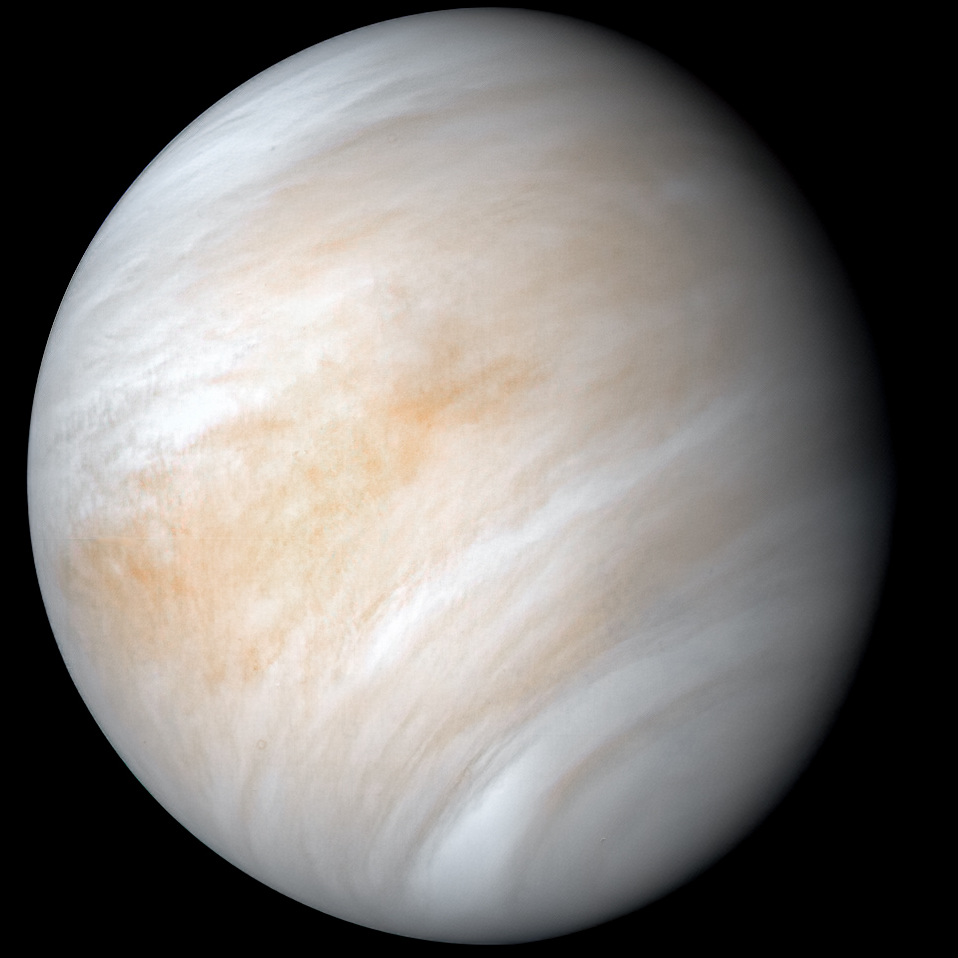
\includegraphics[width=\linewidth]{images/book1/g6-venus-mariner10.jpg}\\[2pt]
{\small शुक्र}
\end{minipage}\hfill
\begin{minipage}[t]{0.31\linewidth}\centering
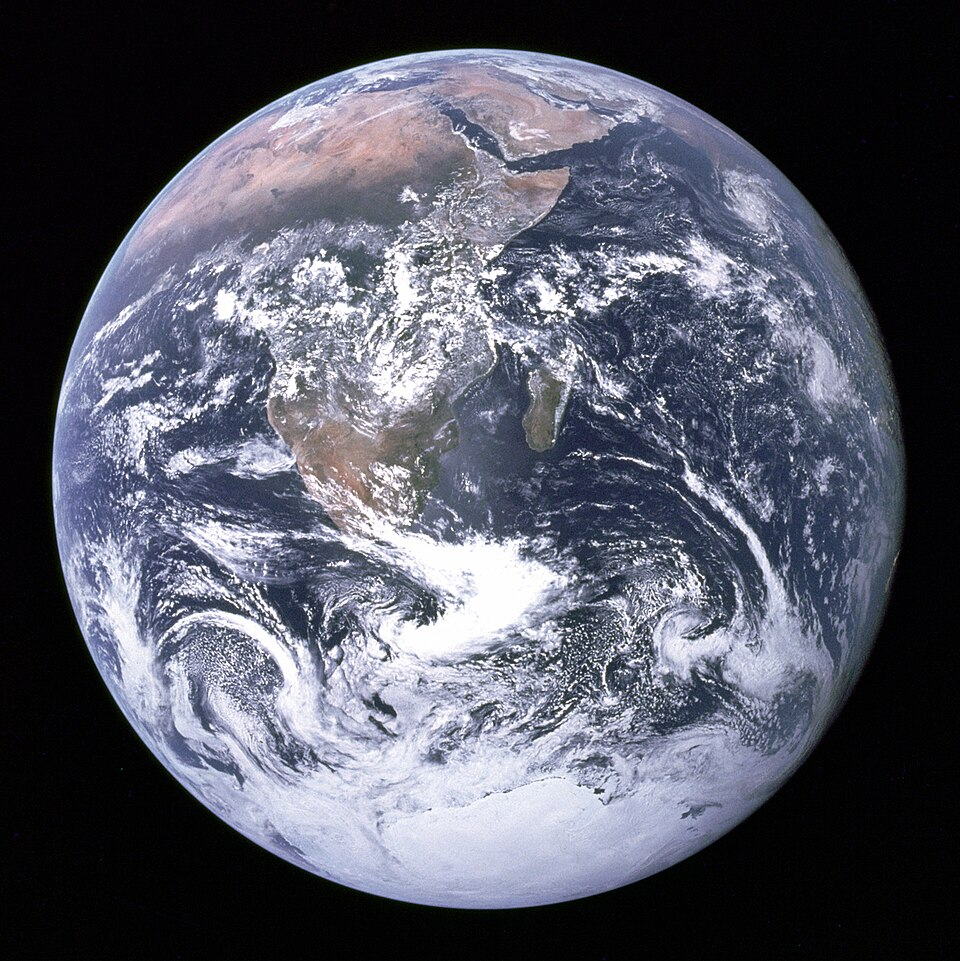
\includegraphics[width=\linewidth]{images/book1/g6-earth-apollo17.jpg}\\[2pt]
{\small पृथ्वी}
\end{minipage}\hfill
\begin{minipage}[t]{0.31\linewidth}\centering
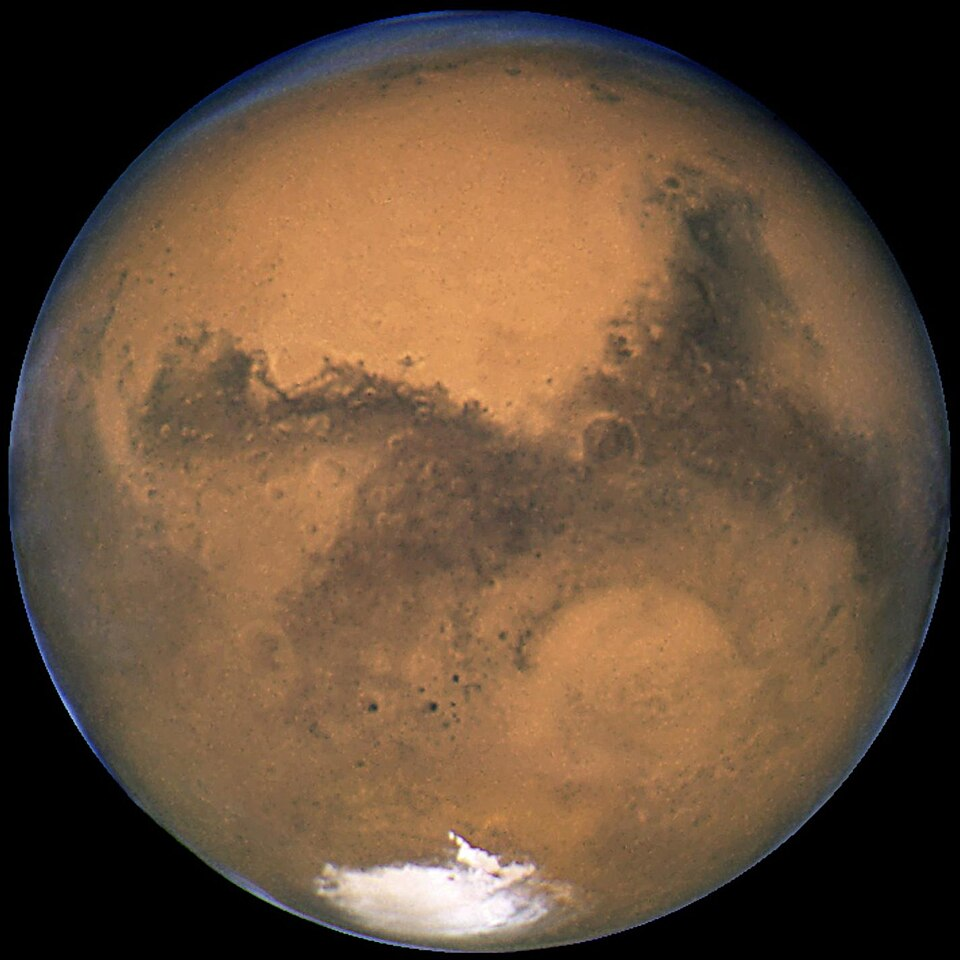
\includegraphics[width=\linewidth]{images/book1/g6-mars-hubble.jpg}\\[2pt]
{\small मंगल}
\end{minipage}

\medskip
{\small अंतरिक्ष से तीन पोस्टकार्ड। शुक्र, जिसका फ़ोटो 1974 में मैरिनर~10 यान ने
खींचा: हमें केवल उसके \omterm{def:g4:clouds-rain-snow:cloud}{बादलों} की ऊपरी सतह दिखती है। पृथ्वी, जिसका फ़ोटो 1972 में
चंद्रमा की ओर जाते हुए अपोलो~17 के दल ने खींचा: सफ़ेद \omterm{def:g4:clouds-rain-snow:cloud}{बादलों} के नीचे अफ़्रीका, अरब
और अंटार्कटिका की बर्फ़। मंगल, जिसका फ़ोटो 2003 में हबल अंतरिक्ष दूरबीन ने खींचा,
अपने \omterm{def:g3:continents-and-oceans:poles}{ध्रुव} पर बर्फ़ की एक सफ़ेद टोपी के साथ।
(फ़ोटो: नासा/JPL-कैलटेक; नासा; नासा, ESA और हबल हेरिटेज टीम।)}
% ledger: nasa:venus-mariner10, nasa:apollo17-earth, hubble:mars-2003
\end{omfigure}

\begin{recall}
भौतिकी की पुस्तकों ने दिखाया कि सूर्य एक तारा है, गरम गैस का एक विशाल गोला जो
अपने-आप चमकता है, और ग्रह एक बड़ा गोल पिंड है जो किसी तारे के चारों ओर घूमता है
और अपने-आप नहीं चमकता: हम उसे इसलिए देखते हैं कि वह अपने तारे का प्रकाश परावर्तित
करता है। सूर्य और उसके चारों ओर घूमने वाली हर चीज़ मिलकर सौर मंडल बनाते हैं। हर ग्रह
सूर्य के चारों ओर एक रास्ते पर चलता है जिसे उसकी कक्षा कहते हैं, और एक अक्ष के चारों
ओर अपने-आप पर घूमता है। हमारे आसपास की हवा हर उस चीज़ पर दबाव डालती है जिसे वह छूती
है: यह वायुदाब है। किसी पदार्थ का घनत्व बताता है कि उसका एक दिया हुआ आयतन कितना
भारी है: एक घन सेंटीमीटर पानी का भार 1~ग्राम है, इसलिए उसका घनत्व 1~ग्राम प्रति घन
सेंटीमीटर है; पानी से ज़्यादा घना पदार्थ उसमें डूबता है, कम घना तैरता है। अंत में, पृथ्वी की सतह के लगभग सात दहाई हिस्से को
\omterm{def:g2:water-on-earth:ocean}{महासागर} ढके हुए है
(\cref{ch:g2:water-on-earth})।
\end{recall}

\section{सूर्य के चारों ओर आठ ग्रह}

आठ ग्रह सूर्य के चारों ओर चलते हैं। क्रम से, सबसे पास से सबसे दूर तक, वे हैं बुध,
शुक्र, पृथ्वी, मंगल, बृहस्पति, शनि, अरुण और वरुण। उनके नामों के पहले अक्षर क्रम
याद रखने में मदद करते हैं: \emph{बु-शु-पृ-मं, बृ-श-अ-व}
(बुध, शुक्र, पृथ्वी, मंगल,
बृहस्पति, शनि, अरुण, वरुण)।

नीचे का चित्र आठों ग्रहों को बगल-बगल में दिखाता है, एक ही पैमाने पर बनाकर: अगर कोई
ग्रह दूसरे से दुगुना चौड़ा है, तो उसका वृत्त भी दुगुना
चौड़ा है।

\begin{omfigure}
\pgfplotstableread{figdata/out/grade-6-planets-sizes.dat}\gsixsizes
\begin{tikzpicture}
  \draw[black!40] (-0.2,0) -- (13.8,0);
  \pgfplotstablegetrowsof{\gsixsizes}
  \pgfmathtruncatemacro{\gsixlast}{\pgfplotsretval-1}
  \foreach \i in {0,...,\gsixlast}{
    \pgfplotstablegetelem{\i}{x_cm}\of\gsixsizes \let\gx\pgfplotsretval
    \pgfplotstablegetelem{\i}{d_cm}\of\gsixsizes \let\gd\pgfplotsretval
    \def\gn{\ifcase\i बुध\or शुक्र\or पृथ्वी\or मंगल\or बृहस्पति\or शनि\or अरुण\or वरुण\fi}
    \pgfplotstablegetelem{\i}{d_km}\of\gsixsizes \let\gk\pgfplotsretval
    \pgfmathsetmacro{\gr}{\gd/2}
    \ifnum\i<4
      \fill[brown!70!black, draw=black!60, line width=0.3pt] (\gx,\gr) circle (\gr);
    \else
      \fill[orange!35, draw=black!60, line width=0.3pt] (\gx,\gr) circle (\gr);
    \fi
    \node[font=\scriptsize, rotate=40, anchor=north east, inner sep=1pt]
      at (\gx+0.08,-0.08) {\gn};
  }
  \node[font=\scriptsize, align=left, anchor=north west] at (-0.2,4.15)
    {\tikz\fill[brown!70!black, draw=black!60] (0,0) circle (2.2pt); चट्टानी ग्रह\\
     \tikz\fill[orange!35, draw=black!60] (0,0) circle (2.2pt); विशाल ग्रह};
  \draw[|-|, black!70] (0,2.2) -- (1,2.2)
    node[midway, above, font=\scriptsize] {35\,000 किमी};
\end{tikzpicture}

{\small पैमाने पर बने आठ ग्रह (व्यास नासा की ग्रह-तथ्य तालिका से)। उनके बीच की
दूरियाँ पैमाने पर नहीं हैं: वे इतनी बड़ी हैं कि किसी भी पृष्ठ पर
नहीं समा सकतीं।}
% ledger: planet:Mercury.diameter, planet:Venus.diameter, planet:Earth.diameter, planet:Mars.diameter, planet:Jupiter.diameter, planet:Saturn.diameter, planet:Uranus.diameter, planet:Neptune.diameter (figdata/grade-6/planets.py, part sizes)
\end{omfigure}

सूर्य के सबसे पास के चार ग्रह छोटे हैं। अगले चार विशाल हैं: बृहस्पति पृथ्वी से लगभग
11 गुना चौड़ा है। और सूर्य? ऊपर के ग्रहों वाले पैमाने पर बनाने पर वह लगभग
40~सेंटीमीटर चौड़ी एक चकती होगा --- इस पृष्ठ से भी
चौड़ी।
% ledger: planet:Jupiter.diameter, planet:Earth.diameter, sun:R (planets.py: sun_cm = 39.9 cm)

आकार ही अकेला अंतर नहीं है। नीचे की तालिका हर ग्रह के लिए उसका व्यास, उसका घनत्व
(ग्राम प्रति घन सेंटीमीटर में), और सूर्य से उसकी दूरी
देती है।

\begin{center}
\small
\begin{tabular}{lrrrr}
\hline
ग्रह & व्यास (किमी) & घनत्व (g/cm$^3$) & सूर्य से दूरी (मिलियन किमी)\\
\hline
बुध & 4\,879 & 5.4 & 58\\
शुक्र & 12\,104 & 5.2 & 108\\
पृथ्वी & 12\,756 & 5.5 & 150\\
मंगल & 6\,792 & 3.9 & 228\\
\hline
बृहस्पति & 142\,984 & 1.3 & 779\\
शनि & 120\,536 & 0.7 & 1\,432\\
अरुण & 51\,118 & 1.3 & 2\,867\\
वरुण & 49\,528 & 1.6 & 4\,515\\
\hline
\end{tabular}
% ledger: planet:Mercury.diameter, planet:Venus.diameter, planet:Earth.diameter, planet:Mars.diameter, planet:Jupiter.diameter, planet:Saturn.diameter, planet:Uranus.diameter, planet:Neptune.diameter, planet:Mercury.density, planet:Venus.density, planet:Earth.density, planet:Mars.density, planet:Jupiter.density, planet:Saturn.density, planet:Uranus.density, planet:Neptune.density, planet:Mercury.dist, planet:Venus.dist, planet:Earth.dist, planet:Mars.dist, planet:Jupiter.dist, planet:Saturn.dist, planet:Uranus.dist, planet:Neptune.dist (figdata/grade-6/planets.py, main table)
\end{center}

घनत्व ग्रहों को दो परिवारों में बाँट देते हैं, बीच में कुछ नहीं: पहले चार घने हैं,
3.9~ग्राम प्रति घन सेंटीमीटर से ज़्यादा, \omterm{def:g3:stones-pebbles-sand:rock}{चट्टान} और धातु की तरह; आख़िरी चार हल्के हैं,
1.7~ग्राम प्रति घन
सेंटीमीटर से कम।

\begin{definition}[चट्टानी ग्रह और विशाल ग्रह]\label{def:g6:earth-a-planet:planet-types}
\emph{चट्टानी ग्रह}\index{चट्टानी ग्रह} एक छोटा, घना ग्रह है जो \omterm{def:g3:stones-pebbles-sand:rock}{चट्टान} और धातु से
बना है, और जिसकी ठोस सतह पर कोई यान उतर सकता है: बुध, शुक्र, पृथ्वी और मंगल।
\emph{विशाल ग्रह}\index{विशाल ग्रह} कम घनत्व वाला एक बहुत बड़ा ग्रह है, जो ज़्यादातर
गैसों और द्रवों से बना है, और जिस पर उतरने के लिए कोई ठोस सतह नहीं: बृहस्पति, शनि,
अरुण और वरुण।
% ledger: nasa:planet-families
\end{definition}

\begin{omfigure}
\begin{minipage}[c]{0.6\linewidth}\centering
\begin{tikzpicture}
  \begin{axis}[ybar, bar width=11pt, width=\linewidth, height=5.4cm,
      ymin=0, ymax=6.2, xmin=-0.6, xmax=7.6,
      xtick={0,...,7}, xticklabels={बुध,शुक्र,पृथ्वी,मंगल,बृहस्पति,शनि,अरुण,वरुण},
      xticklabel style={rotate=40, anchor=north east, font=\scriptsize},
      ytick={0,1,...,6}, ylabel={घनत्व (g/cm$^3$)},
      tick label style={font=\scriptsize}, label style={font=\scriptsize},
      axis x line*=bottom, axis y line*=left]
    \addplot[fill=brown!70!black, draw=black!60, bar shift=0pt, restrict x to domain=0:3]
      table[x=idx, y=density_gcm3] {figdata/out/grade-6-planets-density.dat};
    \addplot[fill=orange!35, draw=black!60, bar shift=0pt, restrict x to domain=4:7]
      table[x=idx, y=density_gcm3] {figdata/out/grade-6-planets-density.dat};
    \draw[blue!60!black, densely dashed] (axis cs:-0.6,1) -- (axis cs:7.6,1);
    \node[font=\scriptsize, blue!60!black, anchor=south, inner sep=1pt]
      at (axis cs:5,1) {पानी};
  \end{axis}
\end{tikzpicture}
\end{minipage}\hfill
\begin{minipage}[c]{0.36\linewidth}\centering
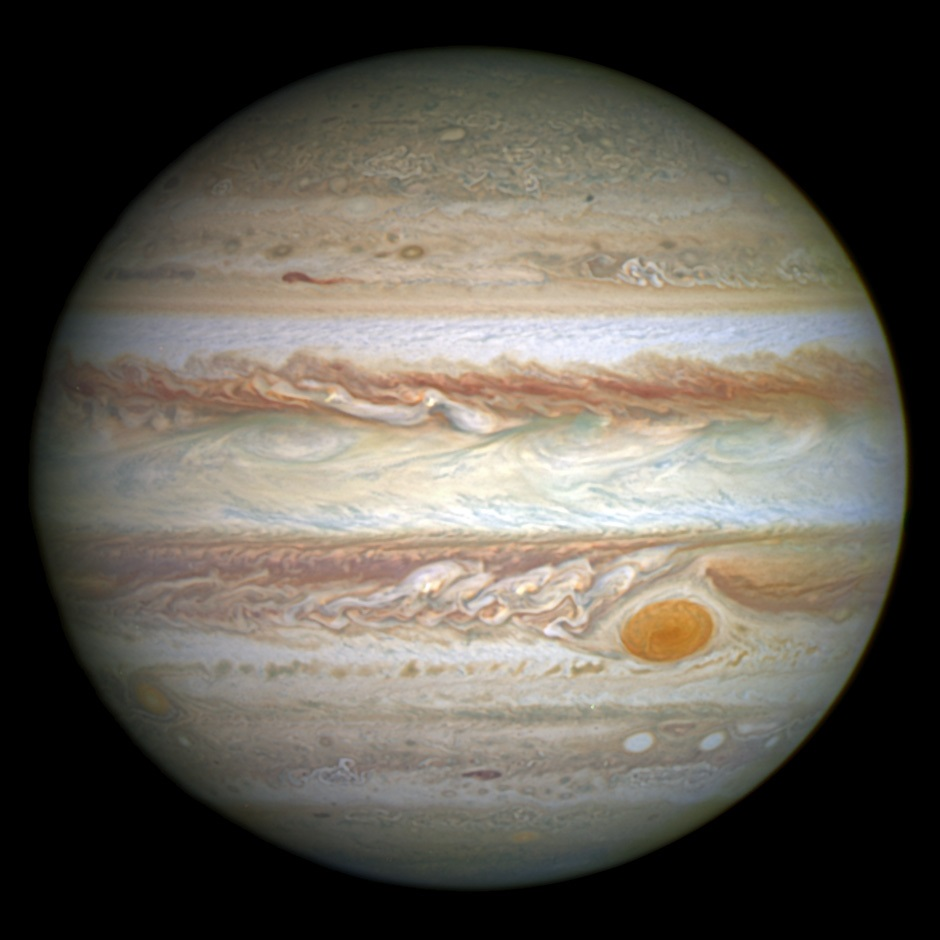
\includegraphics[width=0.9\linewidth]{images/book1/g6-jupiter-hubble.jpg}\\[2pt]
{\small बृहस्पति, जिसका फ़ोटो 2014 में हबल अंतरिक्ष दूरबीन ने खींचा।
(फ़ोटो: नासा, ESA, साइमन।)}
% ledger: hubble:jupiter-2014
\end{minipage}

\smallskip
{\small बाएँ: आठ ग्रहों का घनत्व; धराशायी रेखा पानी का घनत्व है। दाएँ: किसी \omterm{def:g6:earth-a-planet:planet-types}{विशाल
ग्रह} का जो हिस्सा हमें दिखता है, वह उसके \omterm{def:g4:clouds-rain-snow:cloud}{बादलों} की ऊपरी
सतह है।}
% ledger: planet:Mercury.density, planet:Venus.density, planet:Earth.density, planet:Mars.density, planet:Jupiter.density, planet:Saturn.density, planet:Uranus.density, planet:Neptune.density (figdata/grade-6/planets.py, part density)
\end{omfigure}

बृहस्पति के फ़ोटो में \omterm{def:g4:clouds-rain-snow:cloud}{बादलों} की पट्टियाँ दिखती हैं, हल्की और गहरी, और एक लाल अंडाकार
धब्बा: महान लाल धब्बा, पूरी पृथ्वी से भी बड़ा एक विशाल \omterm{def:g5:natural-hazards:storm}{तूफ़ान}, जो सैकड़ों वर्षों से
चल रहा है। \omterm{def:g4:clouds-rain-snow:cloud}{बादलों} के नीचे कोई ज़मीन नहीं है: केवल गैसें, ज़्यादातर हाइड्रोजन और
हीलियम, जो जितनी नीचे जाओ उतनी घनी होती
जाती हैं।
% ledger: nasa:jupiter-gas

\begin{remark}[पानी से हल्का एक ग्रह]\label{rem:g6:earth-a-planet:saturn}
शनि अकेला ग्रह है जिसका घनत्व पानी से कम है: लगभग 0.7~ग्राम प्रति घन
सेंटीमीटर। अगर उसे समा सकने लायक बड़ा कोई बाथटब होता, तो शनि
तैरता!
% ledger: nasa:saturn-float, planet:Saturn.density
\end{remark}

\section{ग्रह एक-दूसरे से कितनी दूर हैं?}

ग्रह केवल आकार में ही बहुत अलग नहीं हैं; वे एक-दूसरे से बहुत दूर भी हैं। पृथ्वी
सूर्य से लगभग 150~मिलियन किलोमीटर दूर है। वरुण, सबसे दूर का ग्रह, 30~गुना ज़्यादा
दूर है: लगभग 4500~मिलियन किलोमीटर। नीचे का चित्र आठों ग्रहों को एक रेखा पर, सूर्य
से उनकी दूरियों पर, पैमाने पर रखता है।
% ledger: planet:Earth.dist, planet:Neptune.dist

\begin{omfigure}
\begin{tikzpicture}
  % whole system
  \draw[thick, gray] (0,0) -- (13.6,0);
  \fill[orange!80!yellow] (0,0) circle (3pt);
  \node[font=\scriptsize, above=3pt] at (0,0) {सूर्य};
  \foreach \n/\x/\lab in {बुध/0.174/, शुक्र/0.326/, पृथ्वी/0.451/, मंगल/0.687/,
                          बृहस्पति/2.345/बृहस्पति, शनि/4.313/शनि, अरुण/8.636/अरुण, वरुण/13.6/वरुण} {
    \fill (\x,0) circle (1.4pt);
    \node[font=\scriptsize, above=3pt] at (\x,0) {\lab};
  }
  \draw[decorate, decoration={brace, amplitude=3pt, mirror}] (0.1,-0.25) -- (0.75,-0.25)
    node[midway, below=3pt, font=\scriptsize, align=center] {चारों\\ चट्टानी ग्रह};
  \draw[<->, thin, gray!70!black] (0,0.62) -- (13.6,0.62) node[midway, above, font=\scriptsize, black] {सूर्य से वरुण तक: लगभग 4500 मिलियन किमी};
  % the inner system, ten times larger
  \begin{scope}[yshift=-2.3cm]
    \draw[thick, gray] (0,0) -- (7.6,0);
    \fill[orange!80!yellow] (0,0) circle (3pt);
    \node[font=\scriptsize, above=3pt] at (0,0) {सूर्य};
    \foreach \n/\x in {बुध/1.744, शुक्र/3.259, पृथ्वी/4.506, मंगल/6.868} {
      \fill (\x,0) circle (1.4pt);
      \node[font=\scriptsize, below=3pt] at (\x,0) {\n};
    }
    \node[font=\scriptsize, anchor=west, align=left] at (8.0,0) {वही रेखा, दस गुना\\ लंबी, चट्टानी ग्रहों के लिए};
  \end{scope}
  \draw[dashed, gray] (0.75,-0.05) -- (7.6,-2.15);
\end{tikzpicture}

{\small सूर्य से ग्रहों की दूरियाँ, पैमाने पर। ऊपर: पूरा सौर मंडल, सूर्य से वरुण
तक। नीचे: चारों \omterm{def:g6:earth-a-planet:planet-types}{चट्टानी ग्रह}, दस गुना बड़े करके। बिंदुओं के आकार पैमाने पर
नहीं हैं।}
% ledger: planet:Mercury.dist, planet:Venus.dist, planet:Earth.dist, planet:Mars.dist, planet:Jupiter.dist, planet:Saturn.dist, planet:Uranus.dist, planet:Neptune.dist (figdata/grade-6/planets.py, part dist)
\end{omfigure}

चारों \omterm{def:g6:earth-a-planet:planet-types}{चट्टानी ग्रह} सूर्य के पास हैं; चारों \omterm{def:g6:earth-a-planet:planet-types}{विशाल ग्रह} दूर बाहर हैं, उनके बीच बहुत बड़े
अंतराल हैं। अकेले मंगल और बृहस्पति के बीच का अंतराल, लगभग 550~मिलियन किलोमीटर, सूर्य से मंगल तक की दूरी के दुगुने से भी ज़्यादा है।
% ledger: planet:Mars.dist, planet:Jupiter.dist

आकार और दूरियाँ एक ही पैमाने पर बनाना कठिन है: ग्रह अदृश्य बिंदु बन जाते हैं। एक
\emph{पैमाना मॉडल} दोनों को एक साथ कल्पना में लाने में मदद करता है।

\begin{method}[सौर मंडल का पैमाना मॉडल बनाना]\label{met:g6:earth-a-planet:scale-model}
\begin{enumerate}
  \item मॉडल में पृथ्वी का आकार चुनो, उदाहरण के लिए 1~cm।
  \item पता करो कि मॉडल का 1~cm कितने असली किलोमीटर के बराबर है: पृथ्वी के असली
        व्यास (12\,756~km) को मॉडल में उसके आकार से भाग दो।
  \item हर असली आकार और हर असली दूरी को इस संख्या से भाग दो।
        फिर इकाइयों को ऐसी चीज़ में बदलो जिसकी कल्पना आसान हो (सेंटीमीटर,
        मीटर, किलोमीटर)।
\end{enumerate}
% ledger: planet:Earth.diameter
\end{method}

\begin{example}[पृथ्वी के लिए एक कंचा]\label{ex:g6:earth-a-planet:marble}
अगर पृथ्वी 1~cm चौड़ा एक कंचा हो, तो 1~cm 12\,756~km के बराबर है। सूर्य,
जिसका व्यास 1\,391\,400~km है, $1\,391\,400 \div 12\,756 \approx
109$~cm चौड़ी एक गेंद बन जाता है: एक छोटे बच्चे से भी ऊँची गेंद। पृथ्वी सूर्य से
150~मिलियन~km दूर है: $149\,600\,000 \div 12\,756 \approx 11\,700$~cm,
यानी लगभग 117~मीटर, एक फ़ुटबॉल के मैदान की लंबाई।
% ledger: planet:Earth.diameter, sun:R, planet:Earth.dist
\end{example}

\begin{center}\small
\begin{tabular}{|l|c|c|}
\hline
\textbf{पिंड} & \textbf{मॉडल में आकार (cm)} & \textbf{सूर्य से दूरी (m)} \\
\hline
सूर्य & 109 & --- \\
बुध & 0.38 & 45 \\
शुक्र & 0.95 & 85 \\
पृथ्वी & 1.00 & 117 \\
मंगल & 0.53 & 179 \\
बृहस्पति & 11.21 & 610 \\
शनि & 9.45 & 1123 \\
अरुण & 4.01 & 2248 \\
वरुण & 3.88 & 3540 \\
\hline
\end{tabular}
\end{center}
% ledger: sun:R, planet:Mercury.diameter, planet:Venus.diameter, planet:Earth.diameter, planet:Mars.diameter, planet:Jupiter.diameter, planet:Saturn.diameter, planet:Uranus.diameter, planet:Neptune.diameter, planet:Mercury.dist, planet:Venus.dist, planet:Earth.dist, planet:Mars.dist, planet:Jupiter.dist, planet:Saturn.dist, planet:Uranus.dist, planet:Neptune.dist (figdata/grade-6/planets.py, part model)

इस मॉडल में वरुण तक का पूरा सौर मंडल 7~km चौड़े एक घेरे पर फैला है, बीच में एक बड़ी
गेंद और उसमें इधर-उधर बिखरे आठ कंचे और गेंदें, जिनमें सबसे बड़ी एक चकोतरे के बराबर
है। सौर मंडल ज़्यादातर ख़ाली
जगह है।

\section{शुक्र, पृथ्वी और मंगल}

शुक्र, पृथ्वी और मंगल पड़ोसी हैं, तीनों \omterm{def:g6:earth-a-planet:planet-types}{चट्टानी ग्रह}। शुक्र लगभग पृथ्वी के बराबर
है: उसका व्यास पृथ्वी के व्यास का 95~\% है। मंगल छोटा है: उसका व्यास पृथ्वी के
व्यास का लगभग आधा है। फिर भी ये तीनों ग्रह इससे ज़्यादा अलग शायद ही हो
सकते थे।
% ledger: planet:Venus.diameter, planet:Earth.diameter, planet:Mars.diameter (planets.py: 94.9 %)

\paragraph{शुक्र।} शुक्र हवा की एक मोटी परत में लिपटा है, जो ज़्यादातर कार्बन
डाइऑक्साइड से बनी है, और जिसमें सल्फ़्यूरिक अम्ल, एक जलाने वाले अम्ल, के घने \omterm{def:g4:clouds-rain-snow:cloud}{बादल}
हैं। उसकी हवा इतनी घनी है कि वह ज़मीन पर उससे 92~गुना ज़ोर से दबाती है जितना
पृथ्वी की हवा हमारी ज़मीन पर। सतह पर तापमान लगभग
464~$^\circ$C है: सीसा पिघलाने लायक गरम। वहाँ कोई पानी
द्रव नहीं रह सकता।
% ledger: nasa:venus-clouds, planet:Venus.psurf, planet:Venus.Tmean

\paragraph{मंगल।} मंगल एक ठंडा, सूखा, धूल भरा \omterm{def:g5:weather-and-climate:desert}{मरुस्थल} है। उसकी हवा भी ज़्यादातर
कार्बन डाइऑक्साइड से बनी है, पर बहुत पतली है: वह ज़मीन पर पृथ्वी की हवा से लगभग सौ
गुना कम दबाती है। औसत तापमान
$-65$~$^\circ$C है। वहाँ आज पानी मिलता है, पर जमा हुआ: ध्रुवीय टोपियों में
बर्फ़ के रूप में और \omterm{def:g3:continents-and-oceans:poles}{ध्रुवों} के पास ज़मीन के नीचे। फिर भी मंगल हमेशा ऐसा नहीं था: अरबों
वर्ष पहले मंगल पर \omterm{def:g1:landscapes-around-us:water}{नदियाँ} बहती थीं, \omterm{def:g1:landscapes-around-us:water}{झीलें} बनती थीं
और \omterm{def:g5:water-shapes-the-land:flood}{बाढ़ें} उसके आर-पार फैलती थीं।
% ledger: nasa:mars-water, planet:Mars.psurf, planet:Mars.Tmean

\paragraph{पृथ्वी।} दोनों के बीच, पृथ्वी की हवा ज़मीन पर लगभग 1~bar से दबाती है
(यह वह इकाई है जिससे ग्रहों पर हवा के दाब की तुलना की जाती है), उसका औसत तापमान
15~$^\circ$C है, और उसके \omterm{def:g2:water-on-earth:ocean}{महासागर}
द्रव पानी के हैं।
% ledger: planet:Earth.psurf, planet:Earth.Tmean

\begin{omfigure}
\begin{tikzpicture}[x=1cm, y=1cm,
    lab/.style={font=\scriptsize, align=center, text width=3.6cm},
    row/.style={font=\scriptsize\bfseries, anchor=east, align=right, text width=2.6cm}]
  % discs to scale: diameters 94.9 %, 100 %, 53.2 % of the Earth's (planets.py)
  \shade[ball color=yellow!60!orange!30] (3,0) circle (0.949);
  \shade[ball color=blue!55] (7,0) circle (1.0);
  \shade[ball color=red!55!brown] (11,0) circle (0.532);
  \node[font=\small\bfseries] at (3,-1.35) {शुक्र};
  \node[font=\small\bfseries] at (7,-1.35) {पृथ्वी};
  \node[font=\small\bfseries] at (11,-1.35) {मंगल};
  \foreach \y/\t in {-2.2/{ज़मीन पर\\हवा का दाब}, -3.2/{औसत\\तापमान},
                     -4.2/{सतह पर\\द्रव पानी}}
    {\node[row] at (1.1,\y) {\t};}
  \foreach \x in {3,7,11}{
    \foreach \y in {-2.2,-3.2,-4.2}{
      \draw[rounded corners=3pt, black!25, fill=black!3] (\x-1.8,\y-0.4) rectangle (\x+1.8,\y+0.4);}}
  \node[lab] at (3,-2.2) {\textbf{92 bar}\\कुचल देने वाला};
  \node[lab] at (7,-2.2) {\textbf{1 bar}};
  \node[lab] at (11,-2.2) {\textbf{0.01 bar}\\बहुत पतली};
  \node[lab, text=red!70!black] at (3,-3.2) {\textbf{464~$^\circ$C}};
  \node[lab] at (7,-3.2) {\textbf{15~$^\circ$C}};
  \node[lab, text=blue!60!black] at (11,-3.2) {\textbf{$-65$~$^\circ$C}};
  \node[lab] at (3,-4.2) {\textbf{नहीं}\\बहुत गरम};
  \node[lab, text=blue!60!black] at (7,-4.2) {\textbf{हाँ}\\महासागर};
  \node[lab] at (11,-4.2) {\textbf{नहीं}\\केवल बर्फ़};
\end{tikzpicture}

{\small शुक्र, पृथ्वी और मंगल की तुलना। तीनों चकतियाँ पैमाने पर बनी हैं।
(मान: नासा की ग्रह-तथ्य तालिका।)}
% ledger: planet:Venus.psurf, planet:Earth.psurf, planet:Mars.psurf, planet:Mercury.Tmean, planet:Venus.Tmean, planet:Earth.Tmean, planet:Mars.Tmean, planet:Jupiter.Tmean, planet:Saturn.Tmean, planet:Uranus.Tmean, planet:Neptune.Tmean, nasa:mars-water
\end{omfigure}

\paragraph{गरम और ठंडा।} सूर्य के पास कोई ग्रह उसका बहुत प्रकाश और ताप पाता है; उससे
दूर, बहुत कम। इसलिए ग्रह सूर्य से जितना दूर हो, उसे उतना ठंडा होना चाहिए। नीचे का
आलेख दिखाता है कि पृथ्वी से बाहर की ओर यह सच है: दूर के \omterm{def:g6:earth-a-planet:planet-types}{विशाल ग्रह} जमी हुई दुनियाएँ
हैं। पर शुक्र को देखो: वह सूर्य से बुध की तुलना में लगभग दुगुनी दूरी पर है, और फिर
भी उससे गरम है! उसकी कार्बन डाइऑक्साइड की घनी हवा सूर्य के ताप को एक भारी कंबल की
तरह फँसा लेती है और उसे निकलने नहीं देती। बुध, जिस पर लगभग कोई हवा नहीं है,
अपना ताप नहीं रख पाता।
% ledger: planet:Mercury.Tmean, planet:Venus.Tmean, planet:Earth.Tmean, planet:Mars.Tmean, planet:Jupiter.Tmean, planet:Saturn.Tmean, planet:Uranus.Tmean, planet:Neptune.Tmean, planet:Mercury.dist, planet:Venus.dist, planet:Earth.dist, planet:Mars.dist, planet:Jupiter.dist, planet:Saturn.dist, planet:Uranus.dist, planet:Neptune.dist, nasa:venus-clouds, planet:Mercury.psurf

\begin{omfigure}
\begin{tikzpicture}
  \begin{axis}[ybar, bar width=14pt, width=0.86\linewidth, height=6cm,
      ymin=-270, ymax=520, xmin=-0.6, xmax=7.6,
      xtick={0,...,7},
      xticklabels={{बुध\\58}, {शुक्र\\108}, {पृथ्वी\\150}, {मंगल\\228},
                   {बृहस्पति\\779}, {शनि\\1432}, {अरुण\\2867}, {वरुण\\4515}},
      xticklabel style={align=center, font=\scriptsize},
      axis x line*=bottom, axis y line*=left,
      xticklabel pos=lower, ytick={-200,-100,...,500},
      ylabel={औसत तापमान ($^\circ$C)}, xlabel={ग्रह और सूर्य से दूरी (मिलियन किमी)},
      tick label style={font=\scriptsize}, label style={font=\scriptsize},
      nodes near coords, nodes near coords style={font=\tiny},
      every node near coord/.append style={/pgf/number format/1000 sep={}}]
    \addplot[fill=orange!50, draw=black!60, bar shift=0pt]
      table[x=idx, y=tmean_C] {figdata/out/grade-6-planets-temp.dat};
    \draw[black!50] (axis cs:-0.6,0) -- (axis cs:7.6,0);
  \end{axis}
\end{tikzpicture}

{\small ग्रहों का औसत तापमान, सूर्य से दूरी के क्रम में। शुक्र नियम तोड़ता है: वह
बुध से गरम है, जो सूर्य के ज़्यादा पास है। (मान: नासा की
ग्रह-तथ्य तालिका।)}
% ledger: planet:Mercury.Tmean, planet:Venus.Tmean, planet:Earth.Tmean, planet:Mars.Tmean, planet:Jupiter.Tmean, planet:Saturn.Tmean, planet:Uranus.Tmean, planet:Neptune.Tmean, planet:Mercury.dist, planet:Venus.dist, planet:Earth.dist, planet:Mars.dist, planet:Jupiter.dist, planet:Saturn.dist, planet:Uranus.dist, planet:Neptune.dist (figdata/grade-6/planets.py, part temp)
\end{omfigure}

\section{पृथ्वी पर जीवन को क्या संभव बनाता है}

पृथ्वी अकेला ग्रह है जहाँ हम जानते हैं कि जीवन है। जीवों को कई परिस्थितियाँ एक साथ
चाहिए, और पृथ्वी के पास वे सब हैं।

\begin{itemize}
  \item \textbf{द्रव पानी।} सभी जीवों को द्रव पानी चाहिए: पृथ्वी पर
        \omterm{def:g2:water-on-earth:ocean}{महासागर}, \omterm{def:g1:landscapes-around-us:water}{नदियाँ} और \omterm{def:g1:landscapes-around-us:water}{झीलें} हैं।
  \item \textbf{हल्के तापमान।} पृथ्वी की सतह पर पानी 0~$^\circ$C पर जमता है
        और 100~$^\circ$C पर उबलता है (भौतिकी)। 15~$^\circ$C के
        औसत के साथ पृथ्वी के तापमान ज़्यादातर इन दोनों के बीच रहते हैं, इसलिए
        उसका पानी द्रव रहता है।
  \item \textbf{सूर्य से सही दूरी।} सूर्य के ज़्यादा पास, शुक्र की तरह, किसी ग्रह के
        बहुत गरम हो जाने का ख़तरा है; ज़्यादा दूर, मंगल की तरह, बहुत
        ठंडा। पृथ्वी द्रव पानी के लिए सही दूरी पर है।
  \item \textbf{एक वायुमंडल।} पृथ्वी के चारों ओर की हवा की परत रात में उसकी
        सतह को गरम रखती है, जीवों को ज़रूरी गैसें देती है, और \omterm{def:g2:water-on-earth:ocean}{महासागरों} पर इतना
        दबाती है कि उनका पानी द्रव रहे। मंगल पर
        हवा इतनी पतली है कि द्रव पानी सतह पर ज़्यादा देर नहीं टिक सकता: वह जम
        जाता है या भाप बन जाता है।
\end{itemize}
% ledger: nasa:mars-water, planet:Earth.Tmean

\begin{remark}[क्या मंगल पर जीवन था?]\label{rem:g6:earth-a-planet:mars-life}
क्योंकि मंगल पर कभी \omterm{def:g1:landscapes-around-us:water}{नदियाँ} और \omterm{def:g1:landscapes-around-us:water}{झीलें} थीं, वैज्ञानिक सोचते हैं कि क्या बहुत पहले, जब
मंगल ज़्यादा गरम और गीला था, वहाँ नन्हे जीव रह सकते थे।
वैज्ञानिकों को आज मंगल पर जीव मिलने की उम्मीद नहीं है; रोबोट
गाड़ियों से वे उसकी \omterm{def:g3:stones-pebbles-sand:rock}{चट्टानों} में बहुत पहले के जीवन के चिह्न खोजते हैं।
% ledger: nasa:mars-water
\end{remark}

\section{अंतरिक्ष से दिखती पृथ्वी}

हज़ारों वर्षों तक लोग केवल कल्पना कर सकते थे कि उनका ग्रह बाहर से कैसा दिखता है।
24~दिसंबर~1968 को, चंद्रमा की कक्षा में घूम रहे अपोलो~8 के अंतरिक्ष यात्रियों ने
चंद्रमा के धूसर क्षितिज के ऊपर पृथ्वी को उगते देखा, और उनमें से एक, बिल एंडर्स, ने
नीचे वाला फ़ोटो खींचा।
% ledger: nasa:earthrise

\begin{omfigure}
\begin{minipage}[c]{0.46\linewidth}\centering
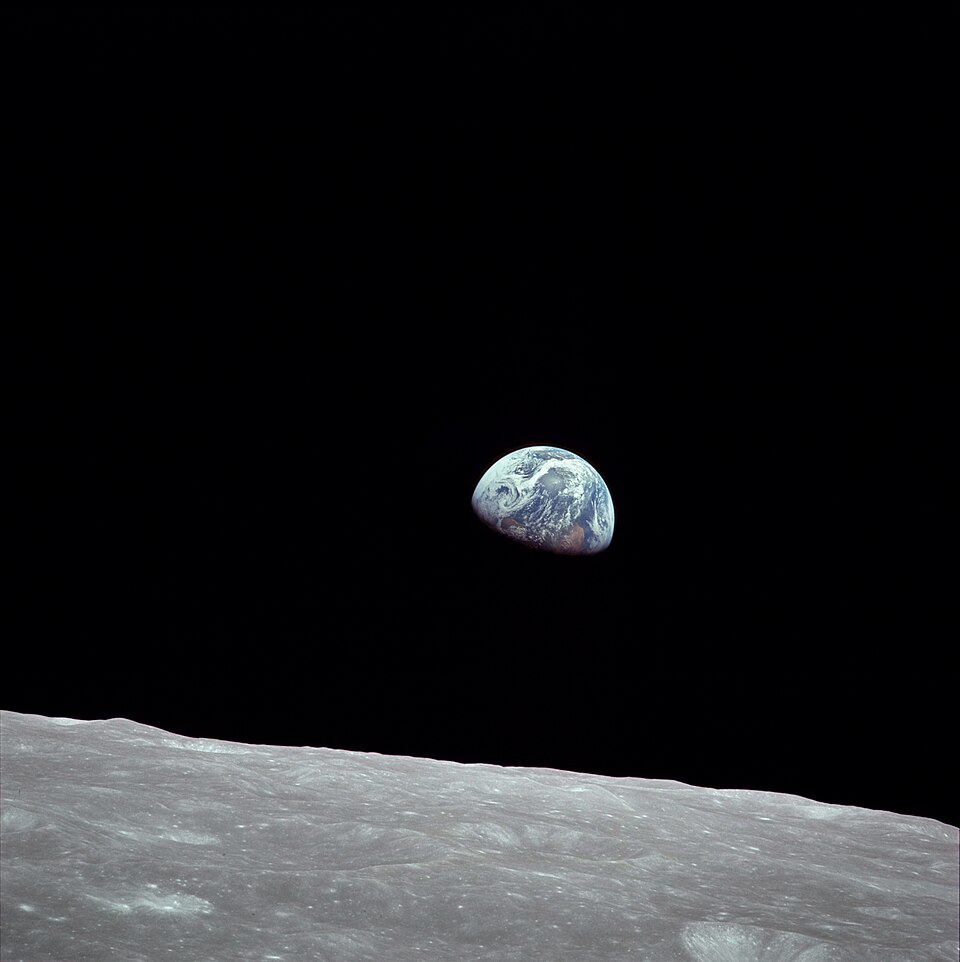
\includegraphics[width=0.85\linewidth]{images/book1/g6-earthrise.jpg}
\end{minipage}\hfill
\begin{minipage}[c]{0.5\linewidth}
{\small \emph{पृथ्वी-उदय}: चंद्रमा के क्षितिज के ऊपर पृथ्वी, चंद्रमा की कक्षा में
घूमते अपोलो~8 से 24~दिसंबर~1968 को खींचा गया फ़ोटो।
(फ़ोटो: नासा, बिल एंडर्स।)}

\medskip
{\small रंगों को देखो: \omterm{def:g2:water-on-earth:ocean}{महासागरों} का नीला, \omterm{def:g4:clouds-rain-snow:cloud}{बादलों} के सफ़ेद भँवर, ज़मीन का भूरा। चारों
ओर अंतरिक्ष का काला; अग्रभूमि में चंद्रमा की बेजान धूसर ज़मीन, बिना पानी और बिना
हवा के।}
\end{minipage}
% ledger: nasa:earthrise
\end{omfigure}

अंतरिक्ष से पृथ्वी ज़्यादातर नीली दिखती है: \omterm{def:g2:water-on-earth:ocean}{महासागर} उसकी सतह के लगभग सात दहाई हिस्से
को ढकता है। उसके ऊपर पानी की बूँदों के सफ़ेद \omterm{def:g4:clouds-rain-snow:cloud}{बादल} भँवर बनाते हैं, और सफ़ेद बर्फ़
\omterm{def:g3:continents-and-oceans:poles}{ध्रुवों} को ढकती है। ज़मीन वहाँ भूरी है जहाँ वह सूखी है, और वहाँ हरी जहाँ पौधे उगते हैं।
हवा ख़ुद नहीं दिखती, पर उसमें तैरते \omterm{def:g4:clouds-rain-snow:cloud}{बादल} दिखाते हैं कि वह है। सौर मंडल के सभी ग्रहों में केवल पृथ्वी ही ये रंग
एक साथ दिखाती है: द्रव पानी, \omterm{def:g4:clouds-rain-snow:cloud}{बादल} और जीवित पौधे।
% ledger: wss:ocean-cover, nasa:apollo17-earth

\begin{history}[फीका नीला बिंदु]
\begin{minipage}[c]{0.66\linewidth}
14~फ़रवरी~1990 को अंतरिक्ष यान वॉयेजर~1 सूर्य से लगभग 6~अरब
किलोमीटर दूर था, वरुण से भी आगे। सौर मंडल को पीछे छोड़ने से पहले उसने अपना कैमरा
पीछे घुमाया और पृथ्वी का एक चित्र खींचा। फ़ोटो में हमारा ग्रह एक अकेला चमकता कण है,
धूल के एक कण से भी छोटा, सूर्य के प्रकाश की एक किरण में फँसा हुआ। खगोलविद कार्ल
सेगन ने उसके बारे में लिखा: ``उस बिंदु को फिर से देखो। वह यहाँ है। वह घर है। वह
हम हैं।''
% ledger: nasa:pale-blue-dot
\end{minipage}\hfill
\begin{minipage}[c]{0.3\linewidth}\centering
\begin{tikzpicture}
  \node[inner sep=0] (img) {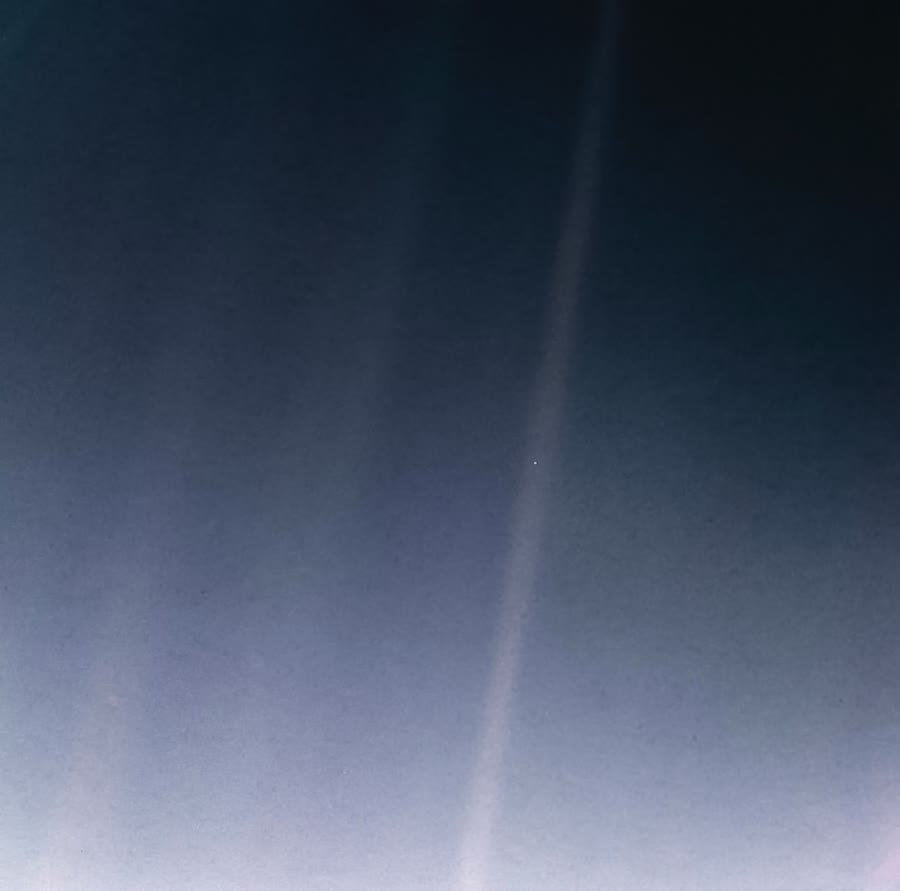
\includegraphics[width=\linewidth]{images/book1/g6-pale-blue-dot.jpg}};
  \draw[yellow!80!orange, thick] ($(img.south west)!0.594!(img.south east) + (0,{0.476*\linewidth})$) circle (6pt);
\end{tikzpicture}\\[2pt]
{\footnotesize वॉयेजर~1 से दिखती पृथ्वी (घेरे में), 1990। (चित्र:
नासा/JPL-कैलटेक, सार्वजनिक डोमेन।)}
% ledger: nasa:pale-blue-dot
\end{minipage}
\end{history}

\section{अभ्यास}

\begin{exercise}[$\star$]\label{exo:g6:earth-a-planet:1}
सौर मंडल के आठों ग्रहों को क्रम से लिखो, सूर्य के सबसे पास वाले से सबसे दूर वाले
तक। \omterm{def:g6:earth-a-planet:planet-types}{चट्टानी ग्रहों} के नीचे रेखा खींचो।
\end{exercise}

\begin{exercise}[$\star$]\label{exo:g6:earth-a-planet:2}
उतारो और पूरा करो: ``\omterm{def:g6:earth-a-planet:planet-types}{चट्टानी ग्रह} छोटा और \ldots{} होता है, जिसकी सतह
\ldots{} होती है। \omterm{def:g6:earth-a-planet:planet-types}{विशाल ग्रह} बहुत बड़ा होता है, कम \ldots{} वाला, जो ज़्यादातर
\ldots{} और \ldots{} से बना होता है।''
\end{exercise}

\begin{exercise}[$\star$]\label{exo:g6:earth-a-planet:3}
इस अध्याय की तालिका की मदद से बताओ: किस ग्रह का व्यास पृथ्वी के व्यास के सबसे पास
है? सबसे बड़ा ग्रह कौन-सा है? सबसे छोटा कौन-सा है?
\end{exercise}

\begin{exercise}[$\star$]\label{exo:g6:earth-a-planet:4}
सही या ग़लत? ग़लत वाक्यों को सुधारो।
(क) शुक्र \omterm{def:g2:water-on-earth:ocean}{महासागरों} से ढका है।
(ख) मंगल पृथ्वी से ठंडा है।
(ग) \omterm{def:g6:earth-a-planet:planet-types}{विशाल ग्रह} सूर्य के सबसे पास के चार ग्रह हैं।
(घ) शनि पानी से कम घना है।
\end{exercise}

\begin{exercise}[$\star\star$]\label{exo:g6:earth-a-planet:5}
बुध का व्यास 4\,879~km है, पृथ्वी का व्यास
12\,756~km। बुध के व्यास को पृथ्वी के व्यास के प्रतिशत के रूप में निकालो,
निकटतम पूर्ण संख्या तक पूर्णांकित करके।
% ledger: planet:Mercury.diameter, planet:Earth.diameter (planets.py: 38.2 %)
\end{exercise}

\begin{exercise}[$\star\star$]\label{exo:g6:earth-a-planet:6}
शनि के व्यास (120\,536~km) के आर-पार कितनी पृथ्वियाँ, बगल-बगल रखकर, समाएँगी?
निकटतम पूर्ण संख्या तक पूर्णांकित करो। शनि \omterm{def:g6:earth-a-planet:planet-types}{चट्टानी ग्रह} है
या \omterm{def:g6:earth-a-planet:planet-types}{विशाल ग्रह}?
% ledger: planet:Saturn.diameter, planet:Earth.diameter
\end{exercise}

\begin{exercise}[$\star\star$]\label{exo:g6:earth-a-planet:7}
खगोलविदों ने दूसरे तारों के चारों ओर ग्रह खोजे हैं। ग्रह~A का घनत्व 1.1~ग्राम
प्रति घन सेंटीमीटर है और वह पृथ्वी से 9~गुना चौड़ा है।
ग्रह~B का घनत्व 5.0~ग्राम प्रति घन सेंटीमीटर है और वह पृथ्वी से थोड़ा
छोटा है। कौन-सा \omterm{def:g6:earth-a-planet:planet-types}{चट्टानी ग्रह} है और कौन-सा \omterm{def:g6:earth-a-planet:planet-types}{विशाल
ग्रह}? समझाओ।
\end{exercise}

\begin{exercise}[$\star\star$]\label{exo:g6:earth-a-planet:8}
ग्रहों के तापमानों के आलेख की मदद से: (क) शुक्र पृथ्वी से कितने डिग्री
ज़्यादा गरम है? (ख) मंगल पृथ्वी से कितने डिग्री
ठंडा है?
% ledger: planet:Venus.Tmean, planet:Earth.Tmean, planet:Mars.Tmean
\end{exercise}

\begin{exercise}[$\star\star$]\label{exo:g6:earth-a-planet:9}
बुध सूर्य के सबसे पास का ग्रह है, पर शुक्र सबसे गरम है। समझाओ
क्यों।
\end{exercise}

\begin{exercise}[$\star\star$]\label{exo:g6:earth-a-planet:10}
पृथ्वी सूर्य से 150~मिलियन किलोमीटर दूर है और मंगल 228~मिलियन
किलोमीटर। मंगल सूर्य से कितने मिलियन किलोमीटर ज़्यादा दूर है? मंगल की दूरी पृथ्वी
की दूरी से कितने प्रतिशत ज़्यादा है (निकटतम पूर्ण संख्या तक
पूर्णांकित करो)?
% ledger: planet:Earth.dist, planet:Mars.dist
\end{exercise}

\begin{exercise}[$\star\star\star$]\label{exo:g6:earth-a-planet:11}
एक दोस्त कहता है: ``मंगल हमेशा से एक सूखा \omterm{def:g5:weather-and-climate:desert}{मरुस्थल} रहा है; वहाँ कभी कोई पानी नहीं
था।'' इस अध्याय की मदद से उसे जवाब दो: अरबों वर्ष पहले मंगल पर क्या था, आज उसका
पानी कहाँ है, और अब उसकी सतह पर द्रव पानी क्यों
नहीं टिक सकता?
\end{exercise}

\begin{exercise}[$\star\star\star$]\label{exo:g6:earth-a-planet:12}
शुक्र को कभी-कभी पृथ्वी का जुड़वाँ कहा जाता है। उसका व्यास पृथ्वी के व्यास का 95~\%
है, और उसकी सतह पर गुरुत्व का खिंचाव एक ऐसे पैमाने पर 8.9 है जिस पर
पृथ्वी का 9.8 है। (क) शुक्र के गुरुत्व के खिंचाव को पृथ्वी के खिंचाव के प्रतिशत के रूप
में निकालो,
निकटतम पूर्ण संख्या तक पूर्णांकित करके। (ख) दो तरीक़े बताओ जिनमें शुक्र पृथ्वी के
जुड़वाँ जैसा है, और दो जिनमें नहीं।
% ledger: planet:Venus.gravity, planet:Earth.gravity, planet:Venus.diameter
\end{exercise}

\section{समस्या: तीन ग्रहों से पोस्टकार्ड}

\begin{problem}[{सप्ताहांत समस्या --- अंतरिक्ष से तीन पोस्टकार्ड, और शुक्र की हवा
उसकी ज़मीन पर कितना दबाती है}]
\label{pb:g6:earth-a-planet:1}
% ledger: planet:Venus.dist, planet:Venus.diameter, planet:Venus.density, planet:Venus.Tmean, planet:Venus.psurf, planet:Earth.dist, planet:Earth.diameter, planet:Earth.density, planet:Earth.Tmean, planet:Earth.psurf, planet:Mars.dist, planet:Mars.diameter, planet:Mars.density, planet:Mars.Tmean, planet:Mars.psurf, nasa:venus-clouds, nasa:mars-water
तीन रोबोट यान घर एक-एक पोस्टकार्ड भेजते हैं, जिनके पीछे कुछ संख्याएँ लिखी
हैं।

\begin{center}
\small
\begin{tabular}{>{\raggedright\arraybackslash}p{0.29\linewidth}>{\raggedright\arraybackslash}p{0.29\linewidth}>{\raggedright\arraybackslash}p{0.29\linewidth}}
\hline
\textbf{शुक्र से} & \textbf{पृथ्वी से} & \textbf{मंगल से}\\
\hline
सूर्य से दूरी: 108~मिलियन~km। & सूर्य से दूरी:
150~मिलियन~km। & सूर्य से दूरी: 228~मिलियन~km।\\
व्यास: 12\,104~km। & व्यास: 12\,756~km। & व्यास: 6\,792~km।\\
घनत्व: 5.2~g/cm$^3$। & घनत्व: 5.5~g/cm$^3$। & घनत्व: 3.9~g/cm$^3$।\\
औसत तापमान: 464~$^\circ$C। & औसत तापमान: 15~$^\circ$C। &
औसत तापमान: $-65$~$^\circ$C।\\
हवा ज़मीन पर 92~bar से दबाती है। अम्ल के घने \omterm{def:g4:clouds-rain-snow:cloud}{बादल}। &
हवा ज़मीन पर 1~bar से दबाती है। \omterm{def:g2:water-on-earth:ocean}{महासागर} और \omterm{def:g4:clouds-rain-snow:cloud}{बादल}। &
हवा ज़मीन पर 0.01~bar से दबाती है। \omterm{def:g3:continents-and-oceans:poles}{ध्रुवों} पर बर्फ़।\\
\hline
\end{tabular}
\end{center}

\medskip
\noindent\textbf{भाग I --- ग्रहों की तुलना।}
\begin{enumerate}
  \item तीनों ग्रहों को सूर्य से दूरी के क्रम में लगाओ।
  \item शुक्र पृथ्वी से कितने मिलियन किलोमीटर ज़्यादा पास है सूर्य के? मंगल कितने
        मिलियन किलोमीटर ज़्यादा दूर है?
  \item मंगल के व्यास को पृथ्वी के व्यास के प्रतिशत के रूप में निकालो,
        निकटतम पूर्ण संख्या तक पूर्णांकित करके। क्या मंगल पृथ्वी की चौड़ाई का लगभग
        एक-चौथाई, आधा या तीन-चौथाई है?
  \item क्या तीनों ग्रह \omterm{def:g6:earth-a-planet:planet-types}{चट्टानी ग्रह} हैं या \omterm{def:g6:earth-a-planet:planet-types}{विशाल ग्रह}? पोस्टकार्डों की कौन-सी
        संख्याएँ तुम्हें यह बताती हैं?
\end{enumerate}

\medskip
\noindent\textbf{भाग II --- हवा।}
\begin{enumerate}[resume]
  \item किस ग्रह पर हवा सबसे घनी है? किस पर वह सबसे
        पतली है?
  \item मंगल की हवा अपनी ज़मीन पर पृथ्वी की हवा की तुलना में हमारी ज़मीन पर
        कितने गुना कम दबाती है?
  \item शुक्र पृथ्वी से ज़्यादा सूर्य के पास है, पर अकेले यह बात
        464~$^\circ$C तापमान को नहीं समझाती। शुक्र की हवा
        सूर्य के ताप के साथ क्या करती है?
  \item शुक्र की ज़मीन पर हवा पृथ्वी की तुलना में कितने गुना ज़ोर से दबाती है?
        शुक्र पर उतरने वाले यान की दीवारें बहुत मज़बूत क्यों होनी चाहिए?
\end{enumerate}

\medskip
\noindent\textbf{भाग III --- पानी और जीवन।}
\begin{enumerate}[resume]
  \item पृथ्वी की सतह पर पानी 0~$^\circ$C पर जमता है और
        100~$^\circ$C पर उबलता है। औसत तापमानों की मदद से समझाओ कि पृथ्वी पर
        पानी द्रव क्यों है।
  \item शुक्र की ज़मीन पर रखे पानी के एक गिलास का क्या होगा? मंगल की
        ज़मीन पर?
  \item मंगल पर अरबों वर्ष पहले \omterm{def:g1:landscapes-around-us:water}{नदियाँ} और \omterm{def:g1:landscapes-around-us:water}{झीलें} थीं। इससे हमें बहुत पहले की मंगल
        की \omterm{def:g5:weather-and-climate:climate}{जलवायु} के बारे में, आज की तुलना में, क्या पता चलता है?
  \item पृथ्वी के पोस्टकार्ड का पिछला हिस्सा लिखो: कुछ वाक्यों में चार कारण बताओ
        कि पृथ्वी पर जीवन क्यों संभव है।
\end{enumerate}
\end{problem}
